The Computer Management console is a Microsoft Management Console (MMC) snap-in that provides a centralized location for managing various system components, services, and settings on Windows. It includes tools for managing disks, services, devices, shared folders, and users, among other administrative tasks.

The console is particularly useful for IT professionals and advanced users who need to perform administrative tasks on local or remote computers.

Om Computer Management te openen zijn er verschillende manieren:
\begin{itemize}
\item
	\begin{enumerate}
		\item Start MMC
		\item Selecteer in het File menu Add/Remove snap-in
		\item Selecteer Computer Management en klik op Add
		\item Voor de lokale machine selecteer Finish
	\end{enumerate}
\item Gebruik de windows-toets + r en run compmgmt.msc
\item Klik op het zoek icoon en zoek op Computer Management
\end{itemize}

\begin{minipage}[t]{\linewidth}
\raggedright
\adjustbox{valign=t}{%
	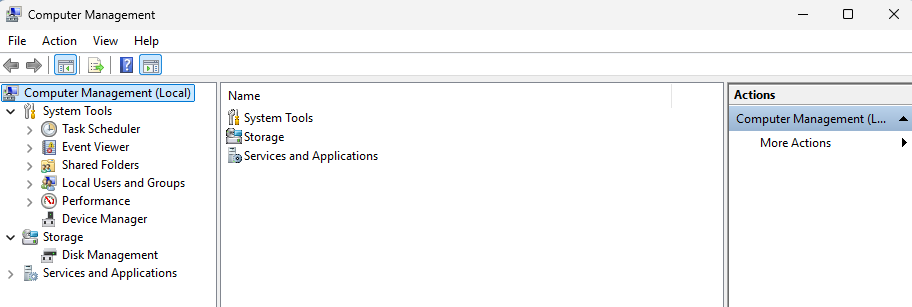
\includegraphics[width=0.99\linewidth]{computermanagement.png}%
}
\end{minipage}

